\section{Evaluering}
\subsection{Test af Korrekthed}
\subsection{Slagterieksempel}
Den simple model, som blev konstrueret til implementering af greenletsversionen, Kan kun bearbejde en gris i konvertering samt en gris i analysen. Dette sikre at det altid er grisen tættest på robotten der får foretaget analysen, men samtidigt betyder det at kun to grise kan konverteres og analyseres samtidigt. Hvis man omvendt tilføjer flere konverterings og analyseprocesser vil der kunne foretages samtidige beregninger, men de enkelte processer vil kæmpe mod hinanden for processesortid uden hensyn til hvilken gris der er nærmest robotten.

Med introduktionen af RTP kan netværket udvides hvis de fysiske rammer for slagteriet ændre sig. Viser det sig f.eks at kameraet holder den samlede produktivitet af netværket tilbage kan, slagteriet tilføjet endnu et kamera, og nemt udvide procesnetværket med endnu en kameraproces, som kan arbejde samtidigt med det første kamera. 
Som programmør kan man også fintune sit netværk og nemt udvide med flere konvertering og analyse processer. Dermed kan programmøren nemt udnytte den underliggende platform. Med RTP sikres at hver gang en proces modtager en gris, bliver det grisen med højst prioritet den modtager, og dette sikre at grisen nærmest robotten først bliver bearbejdet. 
\CRef{fig:pig-network3} viser hvordan netværket kan se ud med flere konverterings og analyse processer. 

\begin{figure}
 \begin{center}
  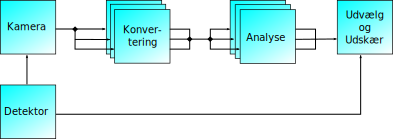
\includegraphics[scale=1]{images/pig-network3}
	\caption{Procesnetværk med flere konverteringsprocesser, og analyseprocesser}
	\label{fig:pig-network3}
\end{center}
\end{figure}


I eksemplet kom vi også ind på at processerne frivilligt skal afgive kontrollen, før robotten kan foretage udskæringen. Med introduktionen af \code{Release} har alle processerne  mulighed for med jævne mellemrum at afgive kontrollen så robotten rettidigt kan foretage selve udskæringen. Hermed skal vi ikke  introducere en delt datastruktur, med de problemer som den har og som vi snakkede om i Barriererafsnittet på side \pageref{sec:barrierer}.
 
